\section{Results and Analysis}

\subsection{Wrong-null verdict flips at MMLU-scale power}
\label{sec:flips}

MMLU-Pro provides the cleanest test. Table~\ref{tab:headline-reference} aligns the chance and best-constant counts under matched point-estimate and interval standards; Table~\ref{tab:mmlupro} in Appendix~\ref{app:mmlupro-and-resort} gives the per-cell values. The reference changes the damaged-arm interpretation, but not every cell moves, so we retain the exact counts rather than claim a universal categorical flip.

\paragraph{Both sides of the flip, held to one standard.}
Those counts were initially asymmetric in evidentiary standard: the floor side carried an interval and a test, whereas ``above chance'' was a bare point comparison. Because both references are deterministic functions of the evaluated item set, the same paired bootstrap can be applied to each side.

\begin{table}[!htbp]
\centering
\scriptsize
\setlength{\tabcolsep}{3pt}
\begin{tabular}{@{}lcc@{}}
\toprule
Scope and standard & Above chance & Above best-constant floor \\
\midrule
MMLU-Pro non-OLMo, point estimate & 10/12 & 3/12 \\
MMLU-Pro non-OLMo, CI$_{95}$ excludes 0 & \textbf{3/12} & \textbf{1/12} \\
MMLU-Pro non-OLMo, BH/Bonferroni at 0.05 & 0/12 & 0/12 \\
Off-MMLU designated OLMo-2 heal cells (25), point est. & 20/25 & 9/25 \\
Off-MMLU designated non-OLMo cells (60), point est. & 25/60 & 4/60 \\
Off-MMLU designated non-OLMo cells (60), CI$_{95}$ excl.\ 0 & --- & 0/60 \\
\bottomrule
\end{tabular}
\caption{\textbf{Calibrating the reference sharply reduces the advertised damaged-arm count.}
The first two rows compare matched point-estimate and paired-bootstrap standards; the third records the
multiplicity result under either stated correction; the final three show
the off-MMLU replication by regime. `Above chance' uses $\mathrm{mean}(1/\texttt{n\_opt})$.
Exact cells and power limits in Tables~\ref{tab:mmlupro} and~\ref{tab:power}. The paired bootstrap
conditions on the observed winning letter; the selection-aware joint resample is \textbf{not run}.}
\label{tab:headline-reference}
\end{table}

The symmetric interval comparison is about one third the size suggested by the asymmetric point-estimate comparison. This does not weaken the reporting rule; it removes an evidentiary mismatch and shows why both the reference and its uncertainty must be stated.

Table~\ref{tab:headline-reference} shows that every interval-level off-MMLU clear belongs to the OLMo-2 rows and aligns the chance, point-floor, and interval-floor counts without repeating them in prose. The item-average convention is operative; the nominal convention would restore the pre-calibration chance-side reading on the MMLU-Pro rows. A joint-resample re-issue is the natural follow-up and must not re-use these counts.

Two qualifications belong with this comparison, both quantified in Appendix~\ref{app:analysis-mult}. McNemar's test does not transfer to a non-binary chance reference, and neither side retains an individual cell after multiplicity correction. The aggregate chance-side count remains unlikely under a global null, so we read it as evidence that the chance side is not uniformly null, not as simultaneously valid per-cell claims.

The result is strong but not universal: 15/17 cells are at or below the floor, and the two exceptions differ in kind. Table~\ref{tab:mmlupro} shows that \texttt{qwen3\_8b\_base/k14} is statistically real but below the materiality gate, whereas OLMo-2 \texttt{shortgpt16} clears its floor decisively. The latter retains more of the stack than any \texttt{keepN} rung, so the floor test does not indiscriminately reject damaged arms (Appendix~\ref{app:designated}).

\paragraph{Materiality is stable against its own threshold.} Figure~\ref{fig:gate-materiality} plots the half-width diagnostic and signed $\Delta_{\mathrm{perm}}$ against the recovery fraction for every cell. The intact Llama-2 anchor fails the precondition, so that family's relative-recovery stack is blocked; Table~\ref{tab:v2-full} supplies the numerator intervals, while $\Delta_{\max}$ is deterministic. Appendix Table~\ref{tab:materiality-diagnostics} reports the full threshold sweep and per-cell diagnostics: the material set is unchanged throughout the intended operating range, and only the lowest sensitivity boundary admits additional cells. Llama-2 remains excluded throughout because its intact anchor fails, not because of post-hoc selection. The table is recomputed from the frozen \texttt{heal\_readout\_v2\_permutation\_null.json} record by \texttt{code/emit\_materiality\_sweep.py}.

The small-benchmark replication contains literal constant emitters that sit on the optimal constant while appearing above chance: the final rows of Table~\ref{tab:headline-reference} show the aggregate supersession of the advertised damaged-arm count. Every surviving above-floor case is a healed \textsc{OLMo-2} arm retaining at least 14 layers; no shallower healed arm or truncate-only arm \emph{significantly} clears its floor. Margins and per-cell counts in Tables~\ref{tab:headline-reference} and~\ref{tab:offmmlu-cells}. Because \textsc{OLMo-2} is the only healed family, this remains a property of that ladder, not a family effect. Appendix~\ref{app:offmmlu} reports the exact constant-emitter, depth, and power counts.

\subsection{Read-out versus retained knowledge}

A floor-level letter score does not imply all task-relevant competence is gone. The ARC-Easy contrast in Table~\ref{tab:diagnostic-contrasts} shows an arm that can rank contents but cannot express that knowledge through the damaged letter interface. Conversely, healthy models often favor letters, so ``content is the fair interface'' generalises no better.

The residual-fraction effect is likewise construct-specific: chance inflates it on OpenBookQA but slightly deflates it on PIQA and ARC-Easy. Null calibration is therefore not a one-way correction; the exact ratios are recorded in Appendix~\ref{app:offmmlu}.

\begin{table}[!htbp]
\centering
\small
\setlength{\tabcolsep}{3.5pt}
\begin{tabular}{@{}p{0.19\linewidth}p{0.24\linewidth}p{0.25\linewidth}p{0.23\linewidth}@{}}
\toprule
Diagnostic & Baseline/read-out & Intervention/contrast & Takeaway \\
\midrule
ARC-Easy \texttt{keep8} & letter 0.2584; floor 0.266414 & content 0.6460; gap $+38.76$ pp & content survives the damaged letter interface \\
Qwen3 \texttt{k8} & v1 $-0.881$ pp ($p=0.0362$) & v2 $-0.139$ pp ($p=0.0964$) & below-floor competence label dissolves \\
Llama-2 \texttt{k8} & v1 $-0.914$ pp ($p=0.0168$) & v2 $-0.416$ pp ($p=0.1002$) & below-floor competence label dissolves \\
OLMo-2 \texttt{keep8}, MMLU & 4,303 bf16 ties; 2,532/14,042 argmax changes & fp32 has zero ties; $\Delta$accuracy $=-0.0015$ & numerical precision does not recover accuracy \\
Qwen3 \texttt{k14} & shipped BH family: 27 cells, $q_{\mathrm{BH}}=0.0297$ & damaged-only family: 23 cells, $q_{\mathrm{BH}}=0.0759$ & multiplicity-corrected downgrade dissolves \\
\bottomrule
\end{tabular}
\caption{\textbf{Representative interventions separate interface failure, arm-conditional signal, and numerical precision.} Full intervals and multiplicity-adjusted results in Tables~\ref{tab:v2-resort} and~\ref{tab:v2-full}.}
\label{tab:diagnostic-contrasts}
\end{table}

\paragraph{V2 re-sorts the 27-cell read-out.}
Under v1, two MMLU-Pro cells are significantly below the best-constant floor; under v2 the below-null count is zero (Table~\ref{tab:diagnostic-contrasts}). V2 is not uniformly conservative: it downgrades \texttt{qwen3/k14} and upgrades \texttt{olmo2/keep14}. The \texttt{qwen3/k14} downgrade survives only under the originally shipped 27-cell BH family and not the pre-declared 23-cell damaged-only family, so we report it as an \emph{uncorrected per-cell observation}. V2 also exposes intact Llama-2-7B as a weak arm-conditional anchor, blocking relative-recovery claims for that family (Table~\ref{tab:v2-resort}).

\begin{figure}[H]
\centering
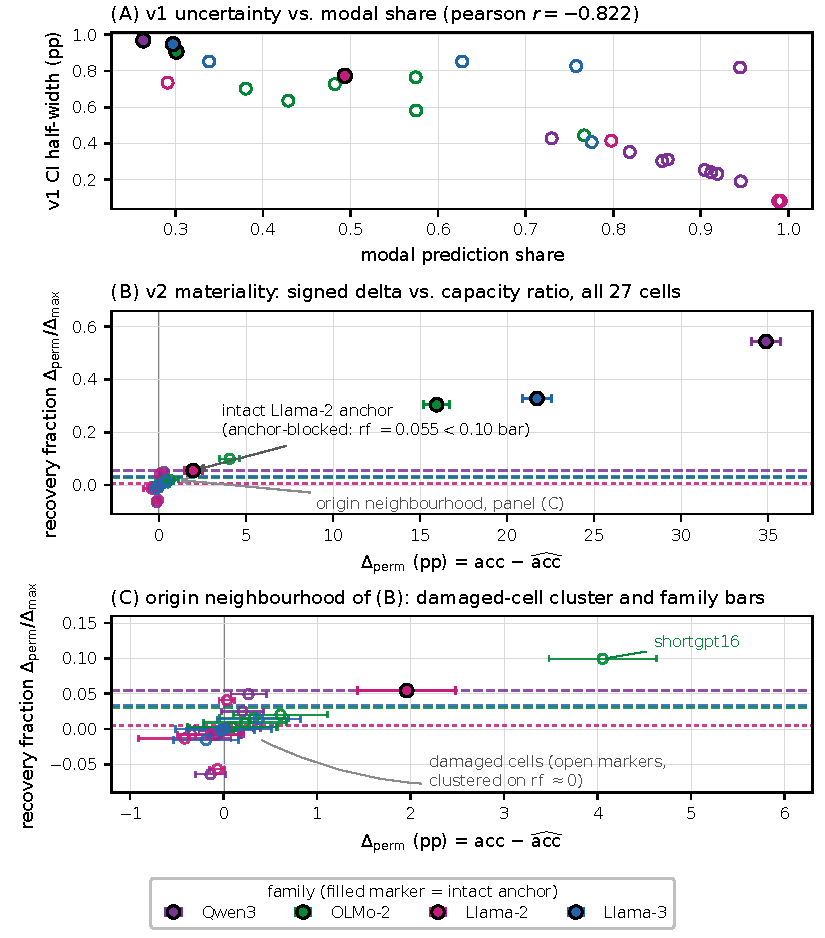
\includegraphics[width=\linewidth]{figures/fig_gate_materiality.pdf}
\caption{\textbf{Quantitative evidence for the gate and its materiality bar (27 cells).}
\textbf{(A)} v1 CI half-width against modal-prediction share (pearson $r=-0.822$;
Table~\ref{tab:v2-full}). \textbf{(B)} signed $\Delta_{\mathrm{perm}}$ against
$r_f=\Delta_{\mathrm{perm}}/\Delta_{\max}$ and the pre-registered family bar.
$\Delta_{\max}$ is deterministic; all 27 rows are in Table~\ref{tab:materiality-diagnostics}.}
\label{fig:gate-materiality}
\end{figure}
